\documentclass[../TDT3.tex]{subfiles}%

\begin{document}

\section[s]"1"{Détente de \textsc{Joule Gay-Lussac}}
\enonce{%
	Le dispositif étudié dans cet exercice a été mis eu point au
	\textsc{xix}\ieme{} siècle par \textsc{Joule} et \textsc{Gay-Lussac} en vue
	d’étudier le comportement des gaz. Deux compartiments indéformables aux parois
	calorifugées communiquent par un robinet initialement fermé. Le compartiment
	(1), de volume $V_1$, est initialement rempli de gaz en équilibre à la
	température $T_i$. Le vide est fait dans le compartiment (2). Une fois le
	robinet ouvert, un nouvel équilibre s’établit, caractérisé par une température
	$T_f$ du gaz.
}%
\QR{%
	Faire un schéma des états initial et final. En considérant comme système fermé
	le contenu des deux compartiments, caractériser la transformation subie par ce
	système.
}{%
	On a le schéma suivant~:
	\begin{center}
		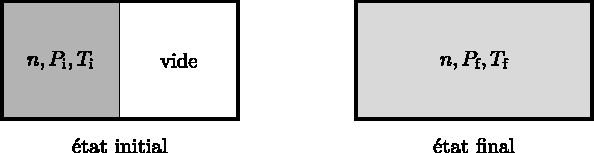
\includegraphics[width=.6\linewidth]{E3_jgl}
	\end{center}
	Pour le système entier, la transformation est \textbf{isochore} car
	parois indéformables, et \textbf{adiabatique} car calorifugées.
}%
\QR{%
	Montrer que cette détente est isoénergétique, c'est-à-dire que l'énergie
	interne du gaz ne varie pas au cours de la transformation. Cette propriété
	dépend-elle du gaz~?
}{%
	Pour le système \{gaz\}, on a $Q = 0$ puisqu'il n'y a pas de trasnfert
	thermique avec l'extérieur ou avec le vide. De plus, $W_p = 0$ puisqu'il n'y a
	pas de force de pression exercée par l'extérieur sur le système. Il n'y a pas
	d'autres travaux. Ainsi, avec le premier principe,
	\[
		\Delta{U} = W + Q
		\Lra
		\boxed{\Delta{U} = 0}
	\]
	Ce résultat \textbf{ne dépend pas du gaz}, qu'il soit réel ou non, puisqu'il
	dépend des propriétés de son environnement uniquement.
}%
\QR{%
	Déterminer la température $T_f$ dans le cas où le gaz est parfait.
}{%
	Comme le gaz est parfait, il suit la première loi de \textsc{Joule}, donc
	\[
		\Delta{U} = C_V\Delta{T}
		\quad \Ra \quad
		\Delta{T} = 0
		\quad \Lra \quad
		\boxed{T_f = T_i}
	\]
}%
\enonce{%
En réalité, on observe une légère diminution de la température du gaz dans la
quasi-totalité des cas. L'expérience est ici réalisée avec du dioxygène, qui
peut être efficacement modélisé par un gaz de \textsc{van der Waals}.
L'équation d'état d'un tel gaz s'écrit
\[
	\left( P + \frac{an^2}{V^2} \right) (V-nb) = nRT
	\qqMath{tel que}
	U = nC_{V,m}T - \frac{an^2}{V}
\]
avec $a$ et $b$ deux constantes positives caractéristiques du gaz. Les travaux
de \textsc{van der Waals} sur le comportement microscopique des gaz ont été de
première importance, et il en a été récompensé par le prix \textsc{Nobel}
1910. Pour le dioxygène, $C_{V,m} = \SI{21}{J.K^{-1}.mol^{-1}}$ et $a =
	\SI{1.32}{USI}$.
}%
\QR{%
% Lalande et Langevin
Interpréter physiquement l'origine du terme de cohésion $a$ et du volume exclu
$b$, et donner leur unité. Nommer et interpréter la constante $C_{V,m}$.
}{%
Le volume exclu $b$ est simple à interpréter~: il traduit qualitativement
l'\textbf{effet du volume occupé par les atomes} du gaz, et qui n'est donc pas
accessible à leur mouvement. Le terme de cohésion lui traduit
l'\textbf{existence de
	forces de \textsc{van der Waals} attractives} entre les atomes de dioxygène.
Ces forces attractives ont pour effet une diminution de la pression au sein
du gaz, ce que traduit bien l'équation d'état~:
\[
	P\sup{GP} = P\sup{\textsc{vdW}} + \frac{an^2}{V^2}
	\Lra
	P\sup{\textsc{vdW}} = P\sup{GP} - \frac{an^2}{V^2} < P\sup{GP}
\]
Pour les unités, on trouve
\[
	[a] = \si{Pa.m^6.mol^{-2}} = \si{J.m^3.mol^{-2}}
	\qqet
	[b] = \si{m^3.mol^{-1}}
\]
Le coefficient $C_{V,m}$ est la \textbf{capacité thermique molaire à volume
	constant} du gaz de \textsc{van der Waals}, $\DS \eval{\pdv{U}{T}}_{n,V} = n
	\cdot C_{V,m}$. C'est l'énergie qu'il faut apporter à \SI{1}{mol} du gaz pour
augmenter sa température de \SI{1}{K}.
}%
\QR{%
	Déterminer l'expression de la température finale $T_f$ du gaz.
}{%
	Avec l'expression de $U$ donnée, comme la transformation reste isoénergétique
	on trouve
	\begin{gather*}
		\Delta{U} =
		nC_{V,m}(T_2-T_i) + an^2 \left( \frac{1}{V_1} - \frac{1}{V_1+V_2} \right) =
		0
		\\\Lra
		T_2 = T_i + \frac{an}{C_{V,m}}\left( \frac{1}{V_1+V_2} - \frac{1}{V_1} \right)
	\end{gather*}
}%
\QR{%
	Effectuer l'application numérique de $\Delta{T}$ pour $n = \SI{0.80}{mol}$ et
	$V_1 = V_2 = \SI{5.0}{L}$.
}{%
	\[
		\xul{\Delta{T} = \SI{-5.06}{K}}
		\qav
		\left\{
		\begin{array}{rcl}
			n         & = & \SI{0.80}{mol}
			\\
			a         & = & \SI{1.32}{J.m^3.mol^{-2}}
			\\
			C_{V,m}   & = & \SI{21}{J.K.mol^{-1}}
			\\
			V_1 = V_2 & = & \SI{5.0e-3}{m^3}
		\end{array}
		\right.
	\]
}%

\end{document}
